\documentclass[a4paper,12pt]{article}
\usepackage{amsmath, amssymb}
\usepackage{xcolor}
\usepackage[most]{tcolorbox}
\usepackage{multicol}
\usepackage{geometry}
\usepackage{graphicx}
\usepackage{hyperref}
\graphicspath{ {../Images/} }

\geometry{left=1.5cm, right=1.5cm, top=2cm, bottom=2cm}


% Style de boîte pour les exercices
\tcbset{
    colframe=purple!70,
    colback=white,
    coltitle=black,
    fonttitle=\bfseries,
    sharp corners,
    boxrule=0.5mm,
    colbacktitle=purple!20!white,
    center title,
    boxsep=4pt,
}

% Style de boîte pour les solutions
\newtcolorbox{solutionbox}[1][]{
    colframe=green!70,
    colback=white,
    coltitle=black,
    fonttitle=\bfseries,
    sharp corners,
    boxrule=0.5mm,
    colbacktitle=green!20!white,
    title=Solution,
    boxsep=4pt,
    breakable,
    #1
}
\begin{document}

% Exercice 15
\begin{tcolorbox}[title={Exercice 15 - {[}Calculer, Représenter{]}}]
Soit les nombres complexes :
\( z_1 = \sqrt{2} + i\sqrt{6} \), \( z_2 = 2 + 2i \) et \( Z = \dfrac{z_1}{z_2} \).
\begin{enumerate}
    \item Écrire \( Z \) sous forme algébrique.
    \item Donner les modules et arguments de \( z_1 \), \( z_2 \) et \( Z \).
    \item En déduire les valeurs de \( \cos \left( \dfrac{\pi}{12} \right) \) et \( \sin \left( \dfrac{\pi}{12} \right) \).
    \item Le plan est muni d’un repère orthonormal. On désigne par \( A \), \( B \) et \( C \) les points d’affixes respectives \( z_1 \), \( z_2 \) et \( Z \). Construire à la règle (non graduée) et au compas les points \( A \), \( B \) et \( C \).
    \item Écrire sous forme algébrique le nombre complexe \( Z^{2022} \).
\end{enumerate}
\end{tcolorbox}

\begin{solutionbox}
\begin{enumerate}
    \item \textbf{Calcul de \( Z \) sous forme algébrique :}

    \[
    Z = \dfrac{z_1}{z_2} = \dfrac{\sqrt{2} + i\sqrt{6}}{2 + 2i} = \dfrac{\sqrt{2} + i\sqrt{6}}{2(1 + i)}
    \]
    
    Pour simplifier, multiplions numérateur et dénominateur par le conjugué de \( 1 + i \), qui est \( 1 - i \) :
    
    \[
    Z = \dfrac{(\sqrt{2} + i\sqrt{6})(1 - i)}{2(1 + i)(1 - i)} = \dfrac{(\sqrt{2} + i\sqrt{6})(1 - i)}{2(1^2 + 1^2)} = \dfrac{(\sqrt{2} + i\sqrt{6})(1 - i)}{4}
    \]
    
    Développons le numérateur :
    
    \[
    (\sqrt{2})(1) - (\sqrt{2})(i) + i\sqrt{6}(1) - i\sqrt{6}(i) = \sqrt{2} - i\sqrt{2} + i\sqrt{6} - i^2 \sqrt{6}
    \]
    
    Comme \( i^2 = -1 \), cela devient :
    
    \[
    \sqrt{2} - i\sqrt{2} + i\sqrt{6} + \sqrt{6}
    \]
    
    Regroupons les termes réels et imaginaires :
    
    \[
    (\sqrt{2} + \sqrt{6}) + i(-\sqrt{2} + \sqrt{6})
    \]
    
    Ainsi :
    
    \[
    Z = \dfrac{ (\sqrt{2} + \sqrt{6}) + i(\sqrt{6} - \sqrt{2}) }{4}
    \]
    
    \item \textbf{Modules et arguments :}

    \textbf{Pour \( z_1 \) :}

    \[
    |z_1| = \sqrt{ (\sqrt{2})^2 + (\sqrt{6})^2 } = \sqrt{2 + 6} = \sqrt{8} = 2\sqrt{2}
    \]

    \textbf{Donc :}
    \begin{align*}
    z_1 &= 2\sqrt{2} \left( \frac{\sqrt{2}}{2\sqrt{2}} + i \frac{\sqrt{6}}{2\sqrt{2}} \right).\\
    &= 2\sqrt{2} \left( \frac{1}{2} + i \frac{\sqrt{3}}{2} \right).
    \end{align*}
    
    \textbf{alors :}
    
    \[
    \arg(z_1) = \dfrac{\pi}{3}
    \]
    
    \textbf{Pour \( z_2 \) :}

    \[
    |z_2| = \sqrt{ 2^2 + 2^2 } = \sqrt{4 + 4} = \sqrt{8} = 2\sqrt{2}
    \]

    \textbf{Donc :}
    \begin{align*}
        z_2 &= 2\sqrt{2} \left( \frac{2}{2\sqrt{2}} + i \frac{2}{2\sqrt{2}} \right).\\
        &= 2\sqrt{2} \left( \frac{\sqrt{2}}{2} + i \frac{\sqrt{2}}{2} \right).
    \end{align*}
    
    \textbf{alors :}
    \[
    \arg(z_2) = \dfrac{\pi}{4}
    \]

    \textbf{Pour \( Z \) :}

    Comme \( Z = \dfrac{z_1}{z_2} \), alors :
    
    \[
    |Z| = \dfrac{|z_1|}{|z_2|} = \dfrac{2\sqrt{2}}{2\sqrt{2}} = 1
    \]
    
    \[
    \arg(Z) = \arg(z_1) - \arg(z_2) = \dfrac{\pi}{3} - \dfrac{\pi}{4} = \dfrac{4\pi - 3\pi}{12} = \dfrac{\pi}{12}
    \]
    
    \item \textbf{Valeurs de \( \cos\left( \dfrac{\pi}{12} \right) \) et \( \sin\left( \dfrac{\pi}{12} \right) \) :}

    Comme \( |Z| = 1 \) et \( \arg(Z) = \dfrac{\pi}{12} \), alors :
    
    \[
    Z = \cos\left( \dfrac{\pi}{12} \right) + i \sin\left( \dfrac{\pi}{12} \right)
    \]
    
    D'après le calcul précédent, nous avons également :
    
    \[
    Z = \dfrac{ (\sqrt{2} + \sqrt{6}) }{4} + i \dfrac{ (\sqrt{6} - \sqrt{2}) }{4 }
    \]
    
    Donc :
    
    \[
    \cos\left( \dfrac{\pi}{12} \right) = \dfrac{ \sqrt{2} + \sqrt{6} }{4}
    \]
    
    \[
    \sin\left( \dfrac{\pi}{12} \right) = \dfrac{ \sqrt{6} - \sqrt{2} }{4 }
    \]
    
    \item \textbf{Construction des points \( A \), \( B \) et \( C \) :}

    Il faut construire les longueurs $\sqrt{2}$ et $\sqrt{6}$. Voici une manière de faire :
    \begin{center}
        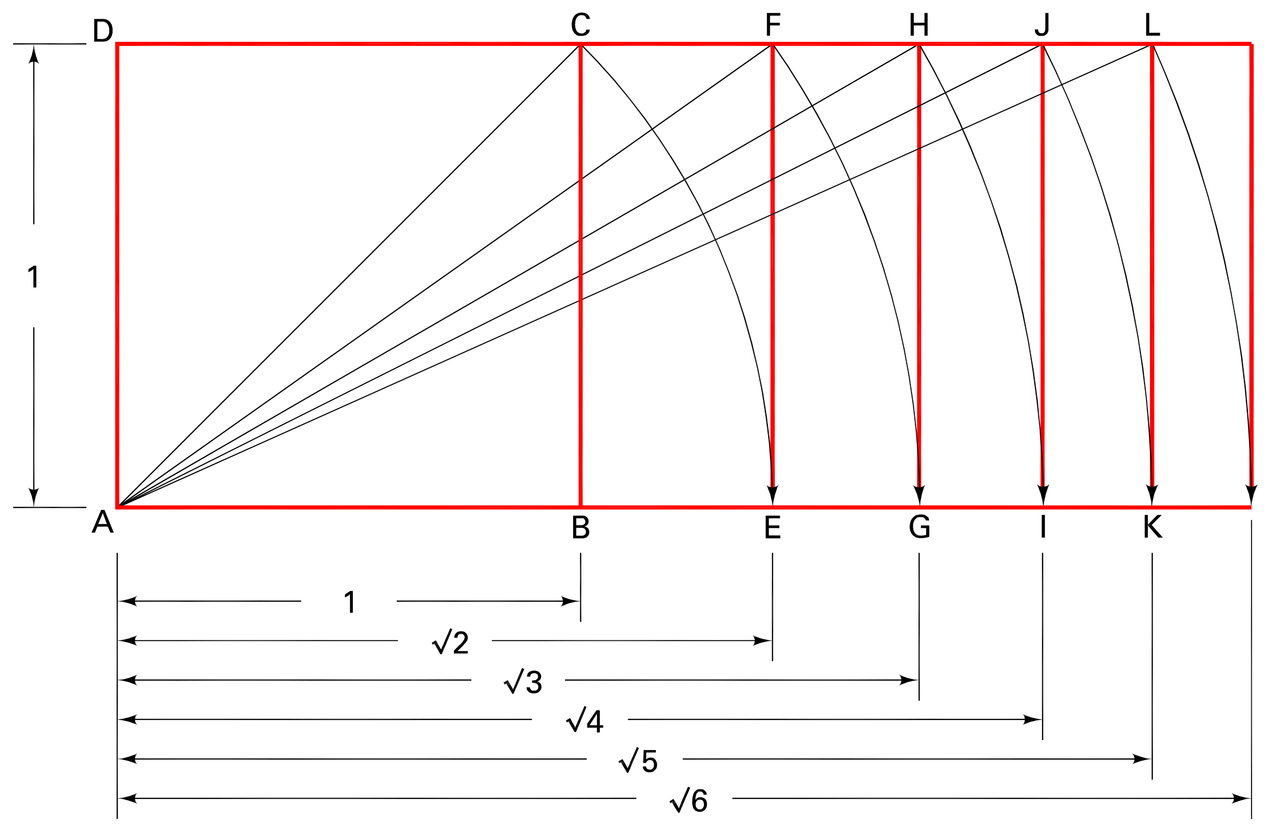
\includegraphics[width=0.8\linewidth]{Root_rectangles_up_to_6.png}
    \end{center}
    
    \item \textbf{Calcul de \( Z^{2022} \) :}

    Puisque \( |Z| = 1 \) et \( \arg(Z) = \dfrac{\pi}{12} \), alors :
    
    \[
    Z^{2022} = e^{i 2022 \times \dfrac{\pi}{12}} = e^{i \dfrac{2022\pi}{12}}
    \]
    
    Simplifions l'argument :
    
    \[
    \dfrac{2022\pi}{12} = \dfrac{2022}{12} \pi = 168.5 \pi
    \]
    
    Comme \( e^{i 2k\pi} = 1 \), nous pouvons soustraire les multiples de \( 2\pi \) :
    
    \[
    168.5 \pi = 84 \times 2\pi + \frac{\pi}{2}
    \]
    
    Donc :
    
    \[
    Z^{2022} = e^{i\frac{\pi}{2}} = i
    \]
    
    \textbf{Conclusion :} \( Z^{2022} = i \)
\end{enumerate}
\end{solutionbox}

\end{document}